\newpage
\section{Wprowadzenie}

Protokół MCP (ang. \textit{Model Context Protocol}) jest standardem \textit{open-source}, udostępnionym przez firmę Anthropic w listopadzie 2024 roku \cite{anthropic-intro}. Według firmy OpenAI stał się najbardziej rozpowszechnionym rozwiązaniem do rozszerzania możliwości modeli AI o dodatkową wiedzę i narzędzia \cite{openai-popularity}. Mimo że nie ma ogólnodostępnego licznika wywołań MCP, liczby takie jak ponad 10 tysięcy aktywnych publicznych serwerów MCP, czy ponad 97 milionów pobranych SDK dla języków Python i TypeScript (stan na 9 grudnia 2025) \cite{anthropic-donating} potwierdzają takie stwierdzenie.

Aby zrozumieć motywację do jego powstania, należy zacząć od dużych modeli językowych (LLM --- ang. \textit{Large Language Models}). Są one rodzajem sieci neuronowych, trenowanych na dużych zbiorach danych do rozwiązywania zadań związanych z przetwarzaniem języka naturalnego. Posiadają jednak istotne ograniczenia. Pierwszym z nich jest ograniczona wiedza. Najbardziej aktualnymi informacjami które model może posiadać są te z momentu jego treningu, nie później. Dzięki temu pierwsze ogólnodostępne modele podawały przestarzałe informacje. Drugim ograniczeniem jest precyzja obliczeń. O ile proste obliczenia mogą być wykonywane poprawnie na podstawie danych treningowych, to przy bardziej złożonych zadaniach LLM-y mają duże problemy.

Powyższe problemy, jak i chęć rozszerzenia możliwości sztucznej inteligencji ponad zwykłe odpowiadania na pytania, zmotywowało deweloperów do pierwszych integracji dużych modeli językowych z zewnętrznymi narzędziami, które mogłyby wykonać problematyczne zadania. Na początku konieczne było pisanie kodu dla każdej pary spośród $M$ modeli AI i $N$ narzędzi, co dawało $M \times N$ integracji (patrz rys.~\ref{fig:mcp-before}). Wykorzystując protokół MCP, każdy model AI musi zaimplementować po jednym i każde narzędzie jeden serwer, co zmniejsza liczbę integracji do $M + N$ (patrz rys.~\ref{fig:mcp-after})~\cite{survey-mcp}.

\begin{figure}[htbp]
    \centering
    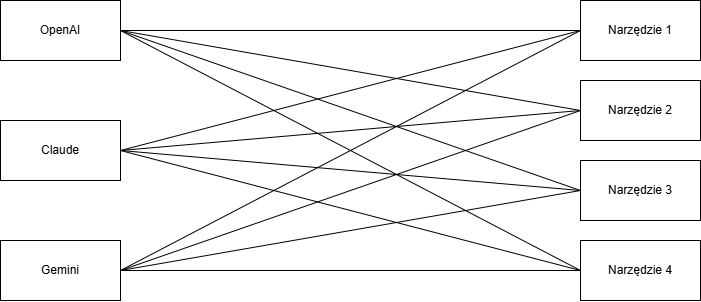
\includegraphics[width=\linewidth]{img/mcp-before.drawio.png}
    \caption{Schemat integracji $M \times N$ (przed protokołem MCP)}
    \label{fig:mcp-before}
\end{figure}

\begin{figure}[htbp]
    \centering
    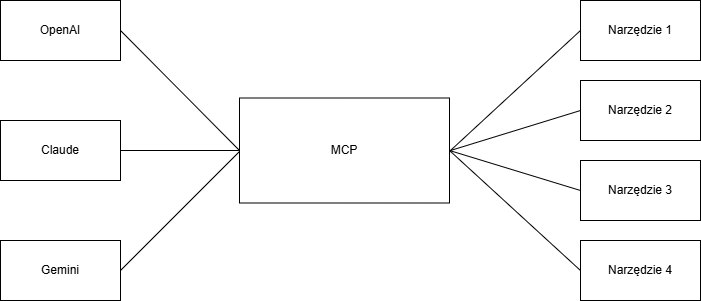
\includegraphics[width=\linewidth]{img/mcp-after.drawio.png}
    \caption{Schemat integracji $M + N$ (wykorzystując protokół MCP)}
    \label{fig:mcp-after}
\end{figure}